\documentclass[a4paper, 12pt]{article}

% Русский язык
\usepackage[T2A]{fontenc}
\usepackage[utf8]{inputenc}
\usepackage[english,russian]{babel}

% Картинки
\usepackage{graphicx}
\graphicspath{{images/}}
\DeclareGraphicsExtensions{.pdf,.png,.jpg}
\usepackage{wrapfig}

% Математика
\usepackage{amsmath,amsfonts,amssymb,amsthm,mathtools} 

% Параметры страницы
\usepackage[left=2cm,right=2cm,top=2cm,bottom=3cm,bindingoffset=0cm]{geometry}

\usepackage{enumitem,xparse}
\usepackage{caption}
\usepackage{subcaption}
\usepackage{float}

\usepackage{hyperref}

\begin{document}

\newgeometry{left=2cm,right=2cm,top=2cm,bottom=1cm,bindingoffset=0cm}

\begin{titlepage}
    \begin{center}

        \vspace*{5cm}

        {\Huge Московский Физико-Технический Институт}\\[2cm]

        {\LARGE Отчёт по эксперименту}\\[0.25cm]

        \noindent\rule{\textwidth}{1pt}
        \vspace*{-0.25cm}

        {\huge \textbf{Энтальпия реакции нейтрализации сильной кислоты сильным основанием}}

        \noindent\rule{\textwidth}{1pt}

        \vfill

    \end{center}

    \begin{flushright}
        \begin{minipage}{0.45\textwidth}
            {\Large
                Выполнил:\\
                Студент 1 курса ФАКТ\\
                Группа Б03-504\\
                Подмосковнов Лев
            }
        \end{minipage}
    \end{flushright}

    \vfill

    \begin{center}
        Долгопрудный\\2026
    \end{center}

\end{titlepage}
\restoregeometry

\setcounter{page}{2}

\subsection*{Цель работы}

Экспериментально определить энтальпию реакции нейтрализации по измерению температуры смеси в ходе реакции.

\subsection*{Реактивы и оборудование}

\begin{itemize}[label=--]
    \item HCl, KOH
    \item Калориметр, термометр
\end{itemize}

\subsection*{Уравнения реакций}
\[
    \text{HCl} + \text{KOH} \rightarrow \text{H}_2\text{O} + \text{KCl}
\]
\[
    \text{H}^+ + \text{Cl}^- + \text{K}^+ + \text{OH}^- \rightarrow \text{H}_2\text{O} + \text{K}^+ + \text{Cl}^-
\]
\[
    \text{H}^+ + \text{OH}^- = \text{H}_2\text{O}
\]

\begin{figure}[H]
    \centering
    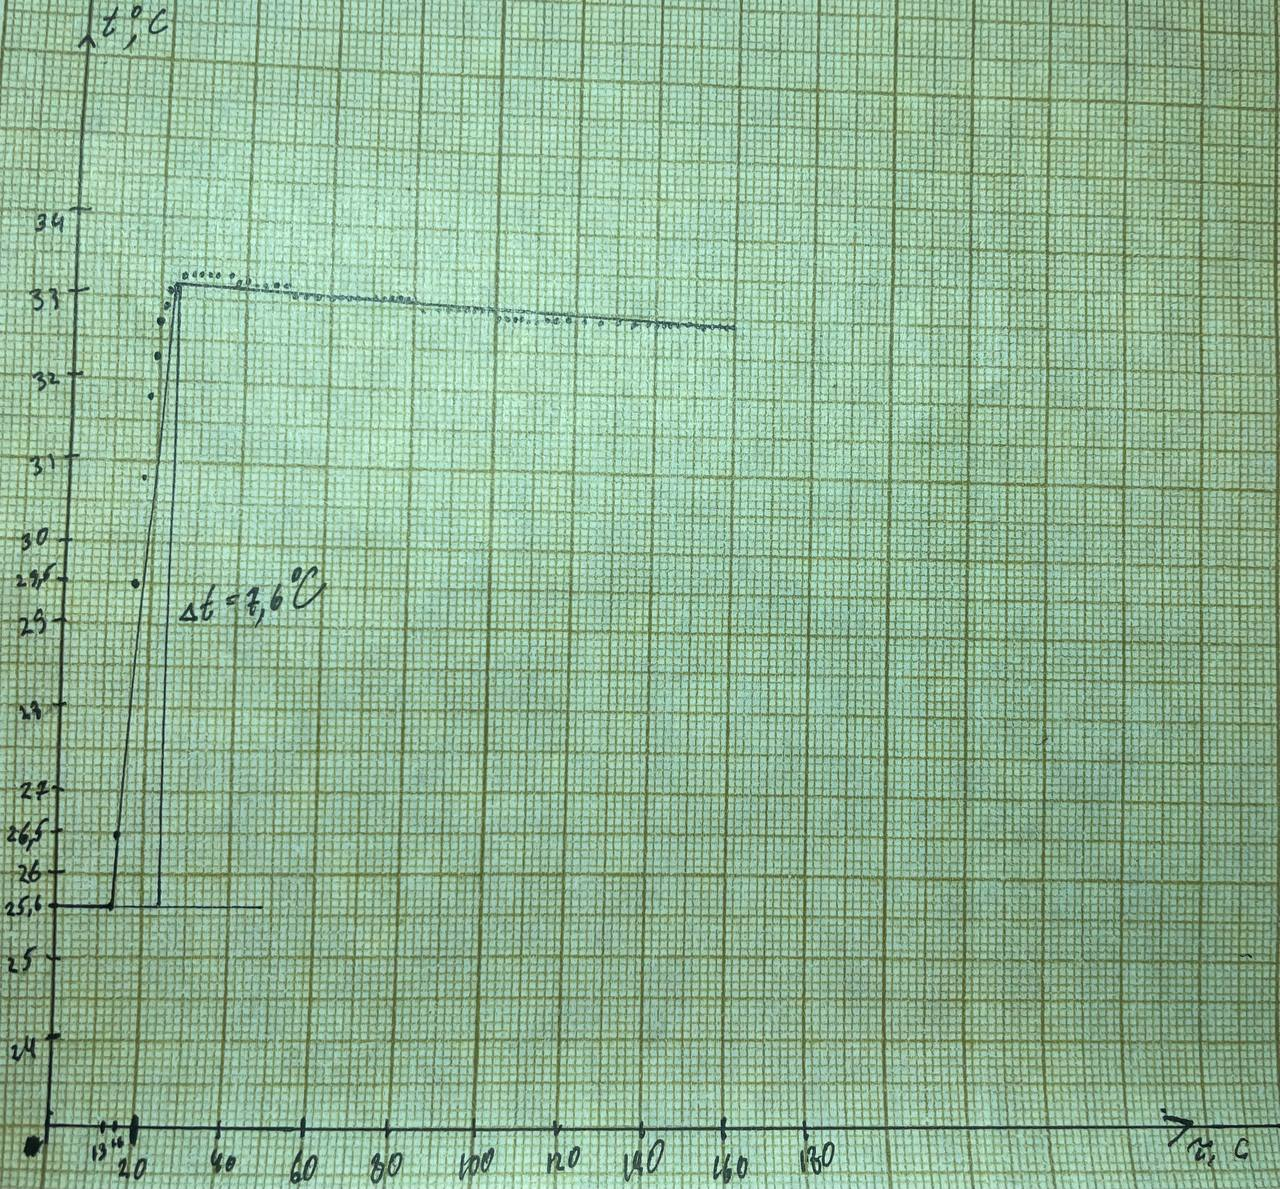
\includegraphics[width=0.9\textwidth]{photo.jpg}
    \caption*{График зависимости температуры от времени}
    \label{fig:temp_graph}
\end{figure}

\newpage

\paragraph{Параметры эксперимента:}
\begin{itemize}[label=--]
    \item Коэффициент калориметра: $k = 0{,}73$
    \item Объем HCl: $V = 100$ мл, $\delta_V = 1$ мл
    \item Объем KOH: $V = 110$ мл, $\delta_V = 1$ мл
    \item Изменение температуры: $\Delta t = 7{,}6^\circ$C (из графика), $\delta_T = 1{,}9^\circ$C
    \item Концентрация HCl: $C_H = 1$ моль/мл
\end{itemize}

\paragraph{Формула для расчета:}
\[
    \Delta H_{\text{впит}} = -\frac{k \cdot \Delta t}{V \cdot C_H}
\]

\paragraph{Расчет:}
\[
    \Delta H_{\text{впит}} = -\frac{0{,}73 \cdot 7{,}6}{0.1 \cdot 1} = -55{,}5 \ \frac{\text{кДж}}{\text{моль}}
\]

\paragraph{Погрешность:}
\[
    \Delta H_{\text{впит}} = -(55{,}5 \pm 1{,}9) \ \frac{\text{кДж}}{\text{моль}}
\]

\paragraph{Табличное значение:}
\[
    \Delta H_{\text{табл}} = -54{,}9 \ \frac{\text{кДж}}{\text{моль}}
\]

\subsection*{Вывод}
Экспериментально была получена энтальпия реакции нейтрализации HCl и KOH. Полученное значение совпадает с табличным в пределах погрешности измерений.

\end{document}